\chapter{Foreign advisors}
\label{chap:advisors}

\section{Description of the framework}
\paragraph{}
We now proceed to definitions associated to the central matter of our thesis, which is the framework for advisory information and its transformations.

\paragraph{}
\definicia Let $M$ be an a-transducer and $L$ a language. Then $M^{-1}(L)$ is the set of all words such, that their images belong to $L$. Formally \\
\centerline{$M^{-1}(L) = \{ w | M(w) \subseteq L \}$.}

\paragraph{}
\definicia Let $L_{dec}$ be a regular language. A pair $(L_{adv}, M)$, where $L_{adv}$ is a regular language and $M$ an a-transducer is called an \emph{advice with regard to $L_{dec}$}, if there exists a deterministic finite automaton $A'$, such that $L_{dec} = L[M^{-1}(L_{adv})](A')$. Moreover, $(L_{adv}, M)$ is called \emph{effective}, if $\C{A'} + \C{M} + \C{L_{adv}} \leq	 \C{L_{dec}}$.

\paragraph{}
\cpriklad Let $L_{dec} = \{ a^{12k}| k \geq 0 \} $, $M$ be one state a-transducer computing the identity and $L_{adv} = \{ a^{2k}| k \geq 0 \}$. $D$ can now construct a simpler finite automaton $A'$ for the language $L_{simple} = \{ a^{6k}| k \geq 0 \}$. Clearly, $\C{A'} + \C{M} + \C{L_{adv}} = 6 + 1 + 2 \leq 12 = \C{L_{dec}}$, which means, that $L_{adv}$ with $M$ is an effective advice with regard  to $L_{dec}$.

\paragraph{}
\cpriklad Let $L_{dec} = \{ a^{12k}| k \geq 0 \} $. Let $M= (\{q_0, q_1\}, \{a\}, \{a\}, H, q_0, \{q_0\})$, where $H = \{(q_0, a, a, q_1), (q_1, a, \varepsilon, q_0)\}$ and $L_{adv} = \{ a^{2k}| k \geq 0 \}$. It is easy to see, that $M^{-1}(L_{adv}) = \{ a^{4k}| k \geq 0 \}$. $D$ can now construct a simpler finite automaton $A'$ for the language $L_{simple} = \{ a^{3k}| k \geq 0 \}$. Clearly, $\C{A'} + \C{M} + \C{L_{adv}} = 3 + 2 + 2 \leq 12 = \C{L_{dec}}$, which means, that $L_{adv}$ with $M$ is an effective advice with regard  to $L_{dec}$.

\paragraph{}
Two interesting questions arise. The first is, for given language $L$ and a-transducer $M$, how to get the language $M^{-1}(L)$? The answer was quite easy to find in previous two examples (and, in fact, for all languages in form $\{ (a^k)^+ \}$ and a-transducers, which just manipulates the number of symbols $a$). The answer in general is resolved by the following Lemma.

\paragraph{}
\clema For an a-transducer $M = (K, \Sigma_1, \Sigma_2, H, q_0, F)$ and a language $L$, $M^{-1}(L) = L'$ if and only if $M(L') = L$ and $\forall w \in L'^c: M(w) = \emptyset \vee M(w) \subseteq L^c$. The mapping $M^{-1}$ can be simulated by an a-transducer $M'$ dual to $M$, such that $M'(L) = L'$ and $\forall w \in L^c: M'(w) = \emptyset \vee M'(w) \subseteq L'^c$. Moreover, $\C{M'} = \C{M}$.

\paragraph{}
\dokaz The first part is quite easy to see, since by definition, $M^{-1}(L)$ contains all words, whose images by a-transducer $M$ belong to $L$. If for a word $v \in L'^c$ there is a word $u$, such that $u \in M(v)$ and $u \notin L^c$, then $u \in L$ and by definition, $v \in L'$, which leads to a contradiction. The proof of the reverse implication is very similar.

\paragraph{}
We prove the second part of our Lemma constructively. Let $M' = (K, \Sigma_2, \Sigma_1, H', q_0, F)$, where\\
\centerline{$H'=\{(p,x,y,q)|(p,y,x,q) \in H\}$.} 

\paragraph{}
Clearly, $\C{M} = \C{M'}$. It remains to show, that $M'$ simulates $M^{-1}$, namely that $M'(L) = L'$ (since $L' = M^{-1}(L)$).
\begin{itemize}
\item $L' \subseteq M'(L)$: Take an arbitrary word $u \in L'$. By definition of $M^{-1}$, there is a word $v \in L$, such that $M(u) = v$. Now, look at the computation of $M$ on $u$ as a word $h \in \Pi_M$ (see Chapter 1). Since this computation is accepting and its output is $v$, we can rewrite $h$ as a sequence of quadruples $(q_0, x_1, y_1, p_1)$ $(p_1,x_2,y_2,p_2)...$ $(p_{i-1},x_i,y_i,p_i)...$$(p_{n-1},x_n,y_n,q_F)$, such that $pr_1(h) = u$ and $pr_2(h) = v$. We now present the computation of $M'$, that show, that $u \in M'(v)$. The computation is $h' \equiv (q_0, y_1, x_1, p_1)$$(p_1,y_2,x_2,p_2)...$ $(p_{i-1},y_i,x_i,p_i)...$$(p_{n-1},y_n,x_n,q_F)$. The plausibility of this computation follows from the construction of $M'$. We have shown, that $u \in M'(L)$ and therefore $L' \subseteq M'(L)$.
\item $M'(L) \subseteq L'$: Once again, let us take a word $u \in M'(L)$. There is a word $v \in L$, such that $u \in M'(v)$. Again, we can look at the respective computation of $M'$ on $v$ as a word $h' \equiv (q_0, y_1, x_1, p_1)$$(p_1,y_2,x_2,p_2)...$ $(p_{i-1},y_i,x_i,p_i)...$$(p_{n-1},y_n,x_n,q_F)$, where $pr_1(h') = v$ and $pr_2(h') = u$. We construct the computation $h$ of $M$ in the same way as in previous part of the proof. The computation $h$ shows, that $v \in M(u)$ and therefore $M(u) \subseteq L$ (whole $M(u)$, since all words $v$, such that $u \in M'(v)$ have to belong to $L$ according to the first part of Lemma). From the definition of $M^{-1}$ it follows, that $u \in M^{-1}(L) = L'$.
\item $\forall w \in L^c: M'(w) = \emptyset \vee M'(w) \subseteq L'^c$: Assume there is a word $w \in L^c$, such that $M'(w) \ni u \wedge u \in L'$. From previous part of Lemma it follows, that $u \in M'(L)$. However, then $w \in M(u) \subseteq L$, which leads to a contradiction.
\end{itemize} \qed

\paragraph{}
Another question is in some sense the inverse perspective of this problem. We have a fixed language $L$ and we want to transform it to a language $L_{adv}$. Since we want to minimize the complexity of the advice, our question is, what is the minimal state complexity of an a-transducer $M$, such that $M^{-1}(L_{adv}) = L$? Previous Lemma has shown us, that this is slightly more difficult thatn the question addressed in Chapter 3, i. e. how to compute $\C{L, L_{adv}}$. However, $\C{L, L_{adv}}$ clearly is a lower bound for $\C{M}$ satisfying aforementioned conditions.

\section{T-decomposable and T-undecomposable languages}

\paragraph{}
\cdefinicia The language $L$ is called \emph{T-decomposable}, if there is a language $L_{adv}$, which is an effective advice for $L$. Otherwise, we call $L$ \emph{T-undecomposable}.

\paragraph{}
Now we to compare our setting to the setting presented by \cite{Gazi} (see Section 2.3). To make the comparison more meaningful, we have to strengthen the condition presented by Gazi in a following way:

\paragraph{}
\cdefinicia A language $L$ is called \emph{A-decomposable}, if there exists an advisor $L_1$ and an automaton $A$, such that $\C{L_1} + \C{A_1} < \C{L}$ and $L(A, L_1) = L$.

\paragraph{}
\cveta Every A-decomposable language is T-decomposable.

\paragraph{}
\dokaz Easy to see, using an a-transducer computing the identity. \qed

\paragraph{}
However, the next theorem shows, that the reverse implication does not hold.

\paragraph{}
\cveta There are infinitely many T-decomposable languages, that are not $\allowbreak$ a-decomposable.

\paragraph{}
\dokaz Such languages are for example $L_{n} = \{ a^n \}$ for $n \geq 10$ and even.

\paragraph{}
We prove this claim in two steps. First, we need to show, that $L_{n}$ is T-decomposable. It is easy to see, that  a DFA accepting $L_{n}$ needs at least $n +2$ states, therefore $\C{L_n} = n + 2$.

\paragraph{}
However, we can use an advice to simplify the accepting automaton as follows: our a-transducer $M$ will encode pairs of letter $a$ into new letters $b$ using two states, where the first state is accepting.

\paragraph{}
Now, the advise language is $L_{n,adv} = \{ b^{\frac{n}{2}} \}$. Clearly, $\C{L_{n,adv}} \leq \frac{n}{2} + 2$.

\paragraph{}
We need to construct just an automaton for $\{a\}^*$, since the advice gives the full information about $L_n$. Altogether, we used $2 + \frac{n}{2}+2+1$ states, therefore for $n \geq 10$ is $L_{n,adv}$ with $M$ an effective advice with regard to $L_n$.

\paragraph{}
Our next goal is to show, that $L_n$ is not A-decomposable. As we have said before, a minimal DFA $A$ for $L_n$ has $n+1$ states and its states correspond to the equivalence classes of the relation defined by Myhill-Nerode theorem (see Section 2.2.1). These equivalence classes are:
\begin{enumerate}
\item $[c_0] = \{ \varepsilon \}$,
\item $[c_{i}] = \{ a^i \}$ for $1 \leq i \leq n$,
\item $[c_{n+1}] = \{ a^k | k > n \}$.
\end{enumerate}

\paragraph{}
We proceed by contradiction, therefore we assume, that we can find an automaton $A'$ and a language $L_{adv}$ (with an automaton $A_{adv}$), such that $\C{A'} + \C{L_{adv}} < \C{L_n} = n+1$. We will show, that both $A'$ and $A_{adv}$ need at least $n$ states, otherwise they would accept an input from $[c_{n+1}]$, which leads to a contradiction, since $\C{A'} + \C{L_{adv}} \geq n+n \geq n+2 = \C{L_n}$.

\paragraph{}
Let us now look at the automaton $A_{adv}$. Since the inequality has to hold, $A_{adv}$ can have at most $n$ states. Also, $A_{adv}$ has to accept the language $L_n$, that means, in our case, the word $a^n$. Clearly, by reading $a^n$, $A_{adv}$ runs in the cycle. Without loss of generality, assume that in one iteration of the shortest cycle $A_{adv}$ reads $a^l$. Therefore, it accepts also incorrect outputs in form of $a^{n + s.l}, s \geq 1$.

\paragraph{}
The same argument can be used for $A'$. Assume, that it accepts also words $a^{n + s.k}, s \geq 1$. However, this means, that $a^{n+s.k.l} \in L_{adv}$ and also $a^{n+s.k.l} \in L(A')$ and our model accepts the word $a^{n + s.k.l}$. However, $a^{n + s.k.l} \notin L_n$.\qed

\paragraph{}
\cdosledok There are infinitely many T-decomposable languages.

\paragraph{}
\cveta There are infinitely many T-undecomposable languages.

\paragraph{}
\dokaz Each of the languages $L_{p} = \{ (a^p)^* | p$ is a prime number $\}$ is T-undecomposable.

\paragraph{}
It is easy to see, that $\C{L_p} = p$. Let us fix a particular $p$ (the arguments will work for all prime numbers $p$, we fix it in order to simplify the notation). We want to decompose $L_p$ to get a simpler automaton $A'$. Let $L_{simple} = L(A')$. Moreover, we will be looking for an advisory language $L_{adv}$ and an a-transducer $M$. Let $L_{trans} = M^{-1}(L_{adv})$.

\paragraph{}
Now, we present some constraints on aforementioned languages. From the definition of the framework, we know, that $L[L_{trans}](A') = L_p$ and therefore $L_p = L_{simple} \cap L_{trans}$. We claim, that $\C{L_{simple}} \geq p$ or $\C{L_{trans}} \geq p$. This can be proven using a series of arguments, which have been already used couple of times in our thesis - since both languages must contain $L_p$ as their subset, if both finite automata have fewer than $p$ states, their computation would run in a cycle of some lengths $k, l$. Then, both automata would accept some word extended by a suitable common multiple of $k$ and $l$ symbols $a$, which however does not belong to $L_p$.

\paragraph{}
On the other side, since we claim, that $L_p$ is T-decomposable, it must hold, that $\C{L_{simple}} \allowbreak < p-1$ (together with another two devices, the total number of states is at most $p$). It follows, that $\C{L_{trans}} \geq p$. What do we know about the complexity of $L_{adv}$? For similar reasons as for $L_{simple}$, also for $L_{adv}$ it has to hold, that $\C{L_{adv}} < p-1$.

\paragraph{}
That means, that in fact, we want to encode the language $L_{trans}$ into the language $L_{adv}$ with a smaller complexity using an a-transducer $M$. However, we not only need, that $M(L_{trans}) = L_{adv}$. Lemma 14 gives us another supplementary conditions on $M$. We want to find two dual a-transducers $M, M'$, such that $M(L_{adv}) = L_{trans}$, $M'(L_{trans}) = L_{adv}$ and both $\C{M} < p$ and $\C{M'} < p$. Besides, $M(L^c_{adv}) \cap L_{trans} = \emptyset$ and $M'(L^c_{trans}) \cap L_{adv} = \emptyset$ (this is just another notation of conditions from Lemma 14).

\paragraph{}
Now, let us consider an a-transducer $M'$ with aforementioned properties and the language $M'(L_{trans})$. We know, that $L_{trans}$ contains all words of the form $(a^p)^*$ and all this words have to be transduced by $M'$ to words from $L_{adv} (M'(L_{trans}))$. Since $M'$ has fewer than $p$ states, the computation of $M'$ on such words contains a cycle. Without loss of generality, take one of the accepting computations on $a^p$ and let the shortest cycle with output have length $c$ (if no cycle has an output, \color{red}lepsi argument je, ze by sme nevedeli generovat dlhsie vystupy\color{black} $M'(a^p) = M'(a^{p+c})$, which violates the condition in Lemma 14). Let the output of this cycle be $x \neq \varepsilon$. Moreover, assume, that the word generated by this computation is $w$.

\paragraph{}
Now, we know, that $w \in L_{adv}$. $M'$ gives correct outputs on all words from $L_{trans}$, so also if we iterate the cycle few more times, we get to the same accepting state.  The substring $x$ can be anywhere in the word $w$, however, without loss of generality, we may assume, that it is in the end. Otherwise the arguments are the same, but with slithly more complex notation. So, we assume $w.(x^{k.p}) \in L_{adv}$ for any $k \geq 0$ (because $w.(x^{k.p}) \in M'(a^{p+k.p.c})$). Consider words of the form $u_i = a^{p+i.c}$ and $v_i = w.(x^i)$ for all $i > 0$. We know, that $v_i \in M'(u_i)$. Using the equivalence relation from Myhill-Nerode theorem (see Section 2), we show, that the number of equivalence classes of $L_{adv}$ is bigger than $p$, which contradicts our assumptions.

\paragraph{}
We claim, that each of the words $v_i$ for $1 \leq i \leq p$ yields another equivalence class. Assume there is a pair of indices $k,l; 1 \leq k < l \leq p$, such that $v_k$ and $v_l$ fall into the same equivalence class. Let $m$ be the smallest number such, that $m>p \wedge v_m \notin L_{adv}$.

\paragraph{}
We will call a number $n$ "bad", if $v_k.(x^{n}) \notin L_{adv}$. We know, that $m-k$ and $m-l$ are bad. For the sake of simplicity, let $r = l-k$. Since $r < p$, at least one of $m-k, m-l$ is not a multiple of $p$. Without loss of generality, let it be $m-k = s$ (the other case is very similar). $v_k$ and $v_l$ are in the same equivalence class, so if $s$ is bad, also $s+r$ is bad. For the same reason, if $s+r$ is bad, also $s+2r$ is bad and all $s+t.r$ for $t \geq 0$ are bad. However, from the group theory we know, that $\Z_p$ is a cyclic group, where every $i \neq 0$ is a generator. Therefore, also $r$ is a generator and for some $j$, $j.r$ is the inverse element to $s+k$. However, this would mean, that $v_{j.r+(s+k)} \notin L_{adv}$, which further means, that $u_{j.r+(s+k)} \in L_{trans}$, while $j.r+(s+k)$ is divisible by $p$, which leads to a contradiction.

\paragraph{}
We need to examine one additional case - if $\forall i, p \leq i: v_i \in L_{adv}$. This means, that $\forall i, p\leq i: u_i = a^{p+i.c} \in L_{trans}$. Though, we have seen, that the automaton $A'$ for $L_{simple}$ has less than $p$ states and again, it runs in a cycle of length $d < p$ when accepting words from $L_{dec}$. Hence a word $a^{p+d.c} \in L_{simple}$. As we have seen, also $a^{p+d.c} \in L_{trans}$, but then $a^{p+d.c} \in L_p$, which is a contradiction, because both $d,c<p$ and $p$ is a prime number. \qed

\paragraph{}
As we have seen, the classes of regular languages concerning T-decomposability are different as the classes of A-decomposable and A-undecomposable languages. In the next part of our thesis, we investigate some properties of these classes.

%------------------------------------------------------------------------------------
\section{Closure properties}

\paragraph{}
When looking at a new class of languages, one of the first natural question, that arises, are its closure properties.  In this section, we want to examine the closure of T-decomposable and T-undecomposable languages under some basic operations and then under deterministic operations presented in \cite{AFDL}.

\subsection{T-undecomposable languages}
\paragraph{}
In this part, we mainly use two types of T-undecomposable languages. First of them are languages of type $L_p = \{ a^{pk} | k \geq 0 \}$ for $p$ a prime number. The T-undecomposability of these languages is proved in previous Section. The second type is a language $L = \{ a \}^*$. This language is clearly undecomposable, since $\C{L} = 1$ and all three devices contained in our foreign advisor concept have non-zero number of states.

\paragraph{}
\cveta The class of T-undecomposable languages is not closed under 
\begin{enumerate}
\item complement,
\item (non-erasing) homomorphism,
\item inverse homomorphism,
\item Kleene star, Kleene plus,
\item intersection,
\item union.
\end{enumerate}

\paragraph{}
\dokaz
\begin{enumerate}
\item \color{red}najst schodny dokaz, posledne dva nevysli\color{black}

\item Consider an undecomposable language $L_1 = \{ a^{13k} | k \geq 0 \}$ and a homomorphism $h:\{ a\}^* \to \{ a \}^*$, such that $h(a) = aa$. Clearly, $h(L_1) = \{ a^{26k} | k \geq 0 \}$ and this language can be decomposed in a following way: let us take an a-transducer $M_1$ computing the identity mapping and a language $L'_1 = \{ a^{2k} | k \geq 0 \}$. This two items form the desired effective advice for $L_1$, since we only have to chceck the language $\{ a^{13k} | k \geq 0 \}$.

Since this homomorphism is non-erasing, our class is not closed even under this kind of mapping.

\item \color{red}ToDo: najst nejaky schopny protipriklad\color{black}

\item \color{red}ToDo: dobra otazka, mozno nakoniec aj bude - ak ma jazyk  tvar $L^*$, potom asi musi byt v automate prechod akceptacny -> pociatocny a tu to vieme roztrhnut a potom ak sa dal zjednodusit ten cely, tak sa musi dat aj ten maly. lenze, tazko povedat, mozno sa ten jazyk tak nejak moze zvrhnut, ze sa to zrazu bude dat rozkladat. zistit!\color{black}

\item Consider two languages, $L_{41} = \{ a^{13k} | k \geq 1 \}$ and $L_{42} = \{ a^{2k} | k \geq 1 \}$. As stated before, both of these languages are T-undecomposable. However, $L_{41} \cap L_{42} = \{ a^{26k} | k \geq 1 \}$ is a T-decomposable language, as we have seen in the first part of this proof.

\item Let us take two languages, $L_{51} = \{ a^k | k \neq 0 (mod 5) \}$ and $L_{52} = \{ a^k | k \neq 0 (mod 7) \}$. The T-undecomposability of these languages can be shown in very similar way, which we have seen in Theorem 17. We show just the first part of the proof, since the rest follows the same pattern as in aforementioned result.

\paragraph{}
Assume, that $L_{51}$ is T-decomposable (the same train of thoughts can be used for $L_{52}$). This means, that we can decompose $L_{51}$ into two languages $L_{trans}$ and $L_{simple}$, such that $L_{trans} \cap L_{simple} = L_{51}$. As we see, $L_{51} \subseteq L_{simple}$. However, since the finite automaton for $L_{51}$ has fewer than $5$ states, it is easy to see, that $L_{simple} \supseteq \{a^*\}$ (otherwise at least one of the words $a, aa, aaa, aaaa$ would be rejected). It  follows, that $L_{trans} \cap \{ a^k | k = 0 (mod 5) \} = \emptyset$. As we  have said, the rest of the proof is almost identical to the proof of Theorem 15.

\paragraph{}
Now we claim, that the language $L_{53} = L_{51} \cup L_{52} = \{a^k|k\neq 0 (mod 35)\}$ is T-decomposable. Clearly, $\C{L_{53}} = 35$. Take the a-transducer $M_5$ from Figure 4.1. It can be seen, that $M_5(a^{5k} = \{ b^k \}$ and $\forall k \neq 5: M_5(a^k) = \{ a^k \}$. Now, let $L_{adv} = \{ w \in \{a,b\}^* | \nexists i: w = b^i \wedge i = 0 (mod 7) \}$. Then, $L_{simple} = \{a\}^*$ and clearly, $(L_{adv},M_5)$ is an effective advice with regard to $L_{53}$.

\begin{figure}
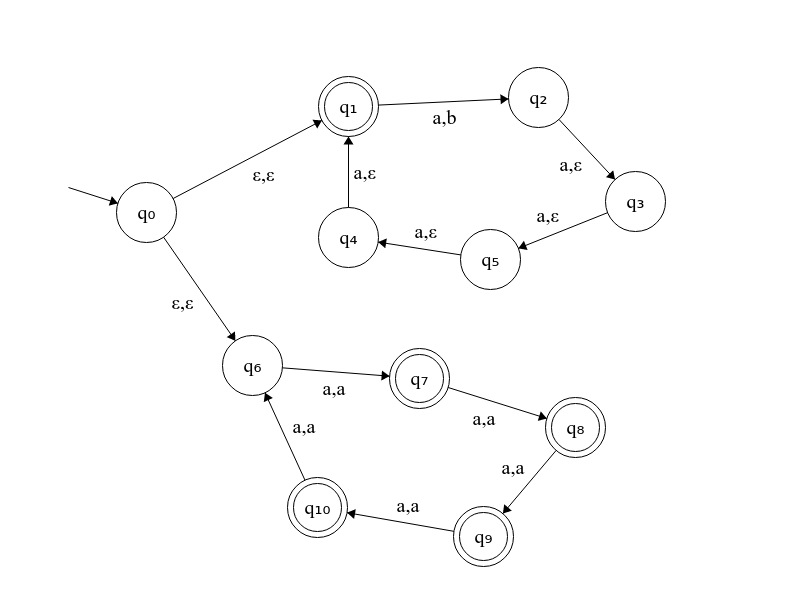
\includegraphics[scale=0.5]{mainmatter/images/M_5.png}
\caption{A-transducer $M_5$}
\end{figure}

\end{enumerate} \qed

\subsection{T-decomposable languages}

\paragraph{}
\cveta The class of T-decomposable languages is not closed under 
\begin{enumerate}
\item complement,
\item (non-erasing) homomorphism,
\item inverse homomorphism,
\item Kleene star, Kleene plus,
\item intersection,
\item union.
\end{enumerate}

\paragraph{}
\dokaz
\begin{enumerate}
\item This claim follows directly from previous Theorem.

\item Let us take a language $L_1 = \{w|w \in \{ a,b\}^* \wedge \#_{a}(w) \mod 42 \equiv 0 \}$. Clearly, a language $L'_1 = \{w|w \in \{ a,b\}^* \wedge \#_{a}(w) \mod 14 \equiv 0 \}$ with an a-transducer $M_1$ computing the identity mapping is an effective advice for $L_1$.

Let us now consider a homomorphism $h: \{ a,b\}^* \to \{ a \}^*$, defined as $h(a) = a, h(b) = a$. Note, that $h$ is a non-erasing homomorphism. It easy to see, that $h(L_1) = \{ a \}^*$, however, as stated before, this language is T-undecomposable.

\item Consider a language $L_2 = \{ a^{26k} | k \geq 1 \}$. The decomposition of this language was shown in the proof of previous theorem. The desired homomorphism is $h: \{a\}^* \to \{a\}^*$, where $h(a) = aa$. Now, $h^{-1}(L_2) = \{ a^{13k} | k \geq 1 \}$, which is T-undecomposable.

\item \color{red}prerobit\color{black}

The counterexample is a language $L_3 = \{ a^{11} \}$. Let us take a language $L'_3 = \{ a^{5} \}$; an a-transducer $M_3 = (\{q_0, q_1, q_2\}, \{a\}, \{a\}, H, q_0, \{q_1\})$, where $H = \{ (q_0, a, \varepsilon, q_1), (q_1, a, \varepsilon, q_2),\allowbreak (q_2, a, a, q_1) \}$; and an automaton $A_3 = (\{q_0\}, \{a\}, \delta, q_0, \{q_0\}) $, where $\delta(q_0, a) = q_0$. Clearly, $M_3^{-1}(L'_3) = L_3$ and $\C{L'_3} + \C{T} + \C{A_3} = 5 + 3 + 1 \leq 9 = \C{L_3}$, therefore $L_3$ is T-decomposable. Though, $(L_3)^+ = \{ a^{11k} | k \geq 1 \}$ and $(L_3)^* = \{ a^{11k} | k \geq 0 \}$ are T-undecomposable.

\item Let us take a look at two languages, $L_{41} = \{ a \}^* \cup \{ b^{15k} | k \geq 1 \}$ and $L_{42} = \{ a\}^* \cup \{ c^{15k} | k \geq 1 \}$. We show the decomposition of $L_{41}$, since that of $L_{42}$ is very similar.

Let $L'_{41} = \{ a\}^* \cup \{ b^{3k} | k \geq 1 \}$ and $M_{41}$ compute the identity mapping. With this advice, we need to check just the language $L''_{41} = \{ a\}^* \cup \{ b^{5k} | k \geq 1 \}$ with an automaton $A''_{41}$. It is easy to see (and provable by Myhill-Nerode theorem), that a DFA for language $L_{41}$ needs at least $18$ states. However, $\C{L'_{41}} + \C{M} + \C{L''_{41}} = 6 + 1 + 8 = 15$ and clearly $L[L'_{41}](A''_{41}) = L_{41}$, which means, that $L_{41}$ is T-decomposable.

However, if we take the language $L_4 = L_{41} \cap L_{42} = \{ a\}^*$, we get a T-undecomposable language, therefore our class is not closed under intersection.

\item In previous section we have seen, that languages $L_{61} = \{a^{10}\}$ and $L_{62}=\{a^{12}\}$ are T-decomposable. Now we show, that also their complements are T-decomposable. Let $M_6 =(\{q_0,q_1,q_2\}, \{a\},\{a,b\},H,q_0,\{q_0,q_2\})$, where $H = \{(q_0,a,\varepsilon,q_1),\allowbreak (q_1,a,b,q_0),\allowbreak (q_0,a,a,q_2)\}$. It can be easily seen, that $M(a^{2k}) = b^k$ and $M(a^{2k+1}) = b^ka$. Now, the effective advice for $L_{61}^c$ consits of $M$ and $L_{61,adv} = \{b^5\}^c$. Clearly, $\C{M} + \C{L_{61,adv}} + \C{\{a\}^*} = 3+7+1 \leq 12 = \C{L_{61}^c}$ and $L_{61}^c = M^{-1}(L_{61,adv}) \cap \{a\}^*$. The effective advice for $L_{62}^c$ can be constructed in the same way.

However $L_{61}^c \cup L_{62}^c = \{a\}^*$ and since $\C{\{a\}^*} = 1$, this language is T-undecomposable.
\end{enumerate} \qed

\subsection{Deterministic operations}
\paragraph{}
As we have seen, the situation with closure propertie of T-decomposable languages is not very interesting. However, this changes, if we are considering the deterministic version of operations (Kleene star/plus, union).

\paragraph{}
\definicia Let $L \subseteq \Sigma^*$ be a language and $c \notin \Sigma$ a new symbol. Then, a \emph{marked Kleene star (plus)} of $L$ is a language $\{ \varepsilon \} \cup L.(cL)^*$ ($L.(cL)^*$). \color{red}[je takato definicia prilis zvrhla? lebo normalna robi trocha problemy s pridavanim pociatocneho stavu]\color{black}. We denote it as $L^{c*} (L^{c+})$.

\paragraph{}
\definicia Let $L_1 \subseteq \Sigma_1^*$ and $L_2 \subseteq \Sigma_2^*$ be languages and $a \notin \Sigma_1$ and $b \notin \Sigma_2$ two new symbols. A \emph{marked union} of $L_1$ and $L_2$ is a language $aL_1 \cup bL_2$.

\paragraph{}
\color{red}ToDo: napisat nejaky vhodny pokec o tom, ze neskumame len jazyk samotny, ale previazany s prekladom (a mozno dokonca s pomocnym jazykom)\color{black}

\paragraph{}
\cveta The class of T-decomposable languages is closed under marked Kleene star/plus.

\paragraph{}
\dokaz Let $L$ be a T-decomposable language with an effective advice $(M, L_{adv})$. Suppose, that we use the advice and check $L$ using an automaton $A_{simple}$. Now consider a language $L' = L^{c*}$. First, we show, that $\C{L'} \geq \C{L}$.

\paragraph{}
Let $A' = (K', \Sigma \cup \{c\}, \delta', q'_0, F')$ be a minimal DFA, such that $L(A') = L'$. Since $A'$ is deterministic, $\forall q' \in F$, there is a transition in form of $\delta(q', c) = p'_{q'}$. 

\paragraph{}
We claim, that for any of aforementioned states $p'_{q'}$, the computation of $A'$ starting in $p'_{q'}$ on a correct input word $w' \in L$ is accepting. Assume this is not the case. Consider the states $q''$ and $p''$, such that $\delta(q'', c) = p''$ and the computation on a word $w$ starting in $p''$ is not accepting. Since $A'$ is minimal and $q''$ is accepting, there is an input $w' \in L'$, such that the computation of $A'$ (with initial state $q'_{0}$) on $w$ ends in $q''$. Now, consider the input $w'cw \in L'$. Since $A'$ is deterministic, $w'cw$ is not accepted, which is a contradiction to the fact, that $L(A') = L'$.


\paragraph{}
Let us pick arbitrary one of $p'_{q'}$ and denote it by $p'$. We can construct an automaton for $L$ as follows: $A = (Q', \Sigma,\delta, \allowbreak p',  F')$, where $\delta = \delta' - \{$transitions on $c \}$. Clearly, as shown in the previous paragraph, $L(A) \subseteq L$. 

\paragraph{}
The reverse containement is easy to see, since if $A$ accepts any word $w \in \Sigma^*$, then also $A'$ accepts this word, but $L(A') \cap \Sigma^* = L$ and $L(A') = L'$, therefore $w \in L$. We see, that  $L(A) \supseteq L$ and together with previous claim it is clear, that $\C{L} \leq \C{L'}$.

\paragraph{}
Now we show the decomposition of $L'$. Let us take $L'_{adv} = L_{adv}^{c*}$. We get the a-transducer $M'$ from $M$ adding transitions $(p, c, c, q_0)$ for each $p \in F$ and $q_0$ the initial state. Now we claim, that the pair $(M', L'_{adv})$ forms an effective advice for $L'$. Clearly, $M'^{-1}(L'_{adv}) = (M^{-1}(L_{adv}))^{c*}$ (since the computation possibilities of the tranducer between markers $c$ are the  same as before) and therefore we only have to check the language $L(A_{simple})^{c*}$.

\paragraph{}
It remains to show that this advice really is effective. To do this, we claim, that for any regular language $R$, $\C{R^{c*}} \leq \C{R}$, since we can get an automaton for $R^{c*}$ by adding $c$-transitions from accepting states to the initial state to the minimal DFA for $R$. Moreover, clearly $\C{M'} = \C{M}$. Therefore, $\C{L^{c*}} \geq \C{L} \geq \C{L_{adv}} + \C{M} + \C{A_{simple}} \geq \C{L'_{adv}} + \C{M'} + \C{A'_{simple}}$ and therefore $\C{L^{c*}} \geq \C{L'_{adv}} + \C{M'} + \C{A'_{simple}}$. \qed
